%#BIBTEX semiautotex.sh -b note_LF_DEM
\documentclass[12pt]{article}
\usepackage{amsmath,amssymb}
\usepackage{bm}
%\usepackage{hyperref}
\usepackage[pdftex]{graphicx}	% required for `\includegraphics' (yatex added)
\usepackage{datetime}
\usepackage{natbib}
\usepackage{tabularx}
\usepackage{mathtools}


%\usepackage{bm}% bold math
\usepackage[pdftex,bookmarks,colorlinks]{hyperref}

\oddsidemargin -1.2cm
\evensidemargin -1.2cm
\textwidth 18cm
\headheight 1.0in
\topmargin -3.5cm
\textheight 22cm


\bibliographystyle{unsrtnat}
\newcommand{\figref}[1]{\figurename ~\ref{#1}}
\newcommand{\tens}[1]{\bm{\mathsf{#1}}}
\title{Simulation model for concentrated suspension\\
\emph{lubrication} and \emph{contact force}}
\date{\shortdate\today \, \ampmtime }
\author{R. Seto, R. Mari}
\usepackage{color}	% required for `\textcolor' (yatex added)
\begin{document}
\maketitle

\section{Targets}

\paragraph{Contact forces}

Friction, rolling friction, cohesion,
these contact forces might have some influence 
of suspension rheology.
%
We may expect that
such contact forces tend to glow up
force correlation (force chains).
%

\paragraph{Criteria of particle contact}

It becomes a question that how 
particles can get in contact 
when lubrication forces act between particles in sheared suspensions.
%
\begin{equation}
\bm{F}_{\mathrm{lub}} = -\frac{1}{4h} (\bm{v}_i-\bm{v}_j)\cdot\bm{n}\bm{n}
\end{equation}
%
This factor $1/h$ is drastic.
%
However, it is not Coulomb type repulsive force.
%
The divergence factor $1/h$
is in the resistance coefficient.
%
Even if the distance is nearly zero $h \ll 1$,
the lubrication force can be small
if the normal element of the relative velocity is samll.
%

In sheared suspensions,
gaps between particles can become very small.
%
If they are perfect spheres,
these gaps are finite positive mathematically.
%
In real system, particles can be get into contact
due to various factors of reality.
%
We need to introduce some persuasive manner 
to allow the direct contact in simulation model.
%
We may introduce a parameter to control this nature systematically.
%

%%%%%%%%%%%%%%%%%%%%%%%%%%%%%%%%%%%%%%%%%%%%%%%%%%%%%%%%%%%%%%%%%%%%%%%%%%%%%%%%%%%%%%%%%%%%%%%%%%%%

The replacement of $1/h$ by $1/h'$ is a possible way,
where $h' \equiv r - 2a' $ with $a' < a$.
%
This $ 1/h'$ does not diverge at $h=2a$.
%
But, this modification systematically
affects overall hydrodynamic interaction.
%
This is why this is not the best way.
%

%%%%%%%%%%%%%%%%%%%%%%%%%%%%%%%%%%%%%%%%%%%%%%%%%%%%%%%%%%%%%%%%%%%%%%%%%%%%%%%%%%%%%%%%%%%%%%%%%%%%
We can introduce a cutoff gap $h^{\ast}$.
\begin{equation}
 \alpha(h) =
\begin{dcases}
\displaystyle \frac{1}{4h} , & h > h^{\ast} \\
\displaystyle  \frac{1}{4h^{\ast}} , & h \leq h^{\ast} 
\end{dcases}
\end{equation}


\paragraph{Force chains}

If volume fraction of suspension is the same,
the increase of viscosity can be realized
by efficient configuration of particles.
%
Many particles seem to cooperate for the resistance of flowing.
%
Force chains are the evidence of the cooperation.
%
Chain-like 1D structures in 3D suspension
indicate the efficiency of particles' collaboration.
%
So, understanding the law of shear-induced force chains
is key task to explain shear thickening.

\paragraph{Avoiding ordering}

Shear induces layering or latticed chains \citep{Catherall_2000}.
%
The shear induced order seems to be a simple tendency.
%

In packing problem,
monodisperse smooth spheres tend to order.
%
Poly- or bidispersity can prevent this.

For the case of the shear induced ordering,
we may expect the mixture of different sizes can avoid in some extent.
%
We plan to check this by introducing bi-disperse simulation.
%

\paragraph{Fore-and-aft asymmetry}

\citet{Parsi_1987}


Observation:

Particles in sheared suspensions collide each other.
%
Multi-collisions take place frequently
if concentrated suspensions are sheared.
%
The essential difference 
between multi-collisions and two-body interactions

push, collide, hard core,

pull, not symmetrical


\paragraph{Check for simulations}

How do the results depend on the simulation parameters?

\begin{itemize}
 \item  \texttt{lubmax}: 2.5, 3, 3.5, 4
 \item  \texttt{lubmin}: 0.01, 0.02, 0.03, 0.04,
 \item 

\end{itemize}


Lubrication max 

identify by seeing contact numbers.








\section{Simulation method}

To solve the problems,
we start to work with particle scale simulation.
%
In order to capture some large scale structure
and to keep aggressive investigation,
we plan to introduce a simplified model than Stokesian dynamics.
%
We plan to follow Ball \& Melrose strategy (1995-2004).
%
They introduced lubrication dynamics 
to simulate concentrated suspensions.
%
They took only the leading order terms of 
the two-body lubrication forces,
which diverges at zero gap $h\to 0$.
%
The force balance equations 
($\bm{F}_{\mathrm{H}}+\bm{F}_{\mathrm{B}}+\bm{F}_{\mathrm{C}} = \bm{0}$)
are solved.
%
The benefits of the lubrication dynamics is 
the drastic reduction of the calculation cost from Stokesian dynamics:
(1) we can build the resistance matrix without matrix inversion,
(2) we can solve equation by using sparse matrix algorithm.
%
The limitation is 
it should be valid for only concentrated suspensions.
%

%%%%%%%%%%%%%%%%%%%%%%%%%%%%%%%%%%%%%%%%%%%%%%%%%%%%%%%%%%%%%%%%%%%%%%%%%%%%%%%%%%%%%%%%%%%%%%%%%%%%

The main extension from Ball \& Melrose model (or Stokesian dynamics)
is the introduction of the direct contact forces between particles.
%
We are preparing to combine contact models 
to the lubrication dynamics.
%
We can also introduce bidisperse simulation
to control shear induced ordering,
though we don't know how much we can avoid it.




\section{Previous works}
\subsection*{Ball and Merlose model}

\subsubsection*{Ball-1995}

\citet{Ball_1995} ``Lubrication breakdown in hydrodynamic simulations of concentrated colloids''
reported the difficulty of the simulation including lubrication force.
Their model is FT-level ($6N$-vectors).
\begin{equation}
 \bm{F}_{\mathrm{H}} = - \tens{R} \bm{V}
\end{equation}
is used for the over damped motion.
\begin{equation}
 \bm{F}_{\mathrm{H}} = \bm{F}_{\mathrm{C}} = 0.
\end{equation}
%
The leading order of the pair-wise squeeze hydrodynamic force
was used.
\begin{equation}
 \bm{f}_i = 
- \sum_j \frac{3 \pi \mu}{8 h_{ij}} 
\left\{
(\bm{v}_i - \bm{v}_j)\cdot \bm{n}_{ij}
\right\} \bm{n}_{ij}\label{125344_18Dec12}
\end{equation}
%
They reported the singular results obtained by this model.
%
The minimum gap and viscosity 
depend on simulation detal, such as time step.
%
They concluded
``The ideal problem of smooth hard spheres
in a Newtonian fluid under simple shear appears
to be singular in nature''.
%

%%%%%%%%%%%%%%%%%%%%%%%%%%%%%%%%%%%%%%%%%%%%%%%%%%%%%%%%%%%%%%%%%%%%%%%%%%%%%%%%%%%%%%%%%%%%%%%%%%%%

We are dubious about their modeling.
%
Their lubrication model \eqref{125344_18Dec12}
is not the same as the leading order of \citet{Jeffrey_1992}.

%%%%%%%%%%%%%%%%%%%%%%%%%%%%%%%%%%%%%%%%%%%%%%%%%%%%%%%%%%%%%%%%%%%%%%%%%%%%%%%%%%%%%%%%%%%%%%%%%%%%


%

\subsubsection*{Melrose-1995}

The article by \citet{Melrose_1995}
titled ``\emph{The Pathological Behaviour of Sheared Hard Spheres with Hydrodynamic Interactions}'' also discussed the difficulty with the same level.

\begin{quote}
\emph{The divergent squeeze terms in principle prevent overlap of particles,
 but computations with fured time steps lead to overlap. }
\end{quote}

\subsubsection*{Melrose-1996}

In \citet{Melrose_1996}
titled ``\emph{Continuous shear thickening and colloid surfaces}'',
they moved on the problem of rheology 
by using the model.  



\subsubsection*{Ball-1997}

Simulation method was reviewed  
by \citet{Ball_1997},
titled 
``\emph{A simulation technique for many spheres 
in quasi-static motion under frame-invariant pair drag and Brownian forces}''.

The equation (12) in the paper is 
\begin{equation}
 - \tens{R} (\bm{V}-\bm{V}_0)
 + \bm{F}^{\mathrm{C}}
 + \bm{F}^{\mathrm{B}}
 - \tens{R} \bm{V}_0 = 0
\end{equation}

\begin{quotation}
\emph{
 The final term in Eq.~(12) is often termed the shear tensor. 
Here it is evaluated at the frame-invariant pair level of the basic approximation. 
(If the shear tensor and the matrix R are formulated separately,
 as, for example, in moment expansions, 
it may be that frame invariance is broken and this should be checked for in practice.)
}
\end{quotation}

In Appendix A, more explicit calculations are give.
$\bm{f}_i$ and $\bm{g}_i$ are force and torque acting on particle $i = 1,2$.
\begin{align*}
 \bm{f}_1 & =  -\bm{f}_2 \\
&=- a_{\mathrm{sq}} \tens{N}  (\bm{v}_1 - \bm{v}_2)
- a_{\mathrm{sh}} \left(\frac{2}{r}\right)^2
\tens{P} (\bm{v}_1 - \bm{v}_2)
+ \left(\frac{2}{r}\right) a_{\mathrm{sh}}
\bm{n} \times \tens{P} (\bm{w}_1 + \bm{w}_2) \\
\bm{g}_1 &= 
-\left(\frac{2}{r}\right) a_{\mathrm{sh}}
\bm{n} \times \tens{P}(\bm{v}_1-\bm{v}_2)
- a_{\mathrm{sh}} \tens{P}(\bm{\omega}_1+\bm{\omega}_2)
- a_{\mathrm{pu}} \tens{P}(\bm{\omega}_1-\bm{\omega}_2)
- a_{\mathrm{tw}} \tens{N}(\bm{\omega}_1-\bm{\omega}_2) \\
\bm{g}_2 &= 
-\left(\frac{2}{r}\right) a_{\mathrm{sh}}
\bm{n} \times \tens{P}(\bm{v}_1-\bm{v}_2)
- a_{\mathrm{sh}} \tens{P}(\bm{\omega}_1+\bm{\omega}_2)
+ a_{\mathrm{pu}} \tens{P}(\bm{\omega}_1-\bm{\omega}_2)
+ a_{\mathrm{tw}} \tens{N}(\bm{\omega}_1-\bm{\omega}_2)
\end{align*}
where $\tens{N} = \bm{n}\bm{n}$,
$\tens{P} =1- \bm{n}\bm{n}$,
and 
$r = d + h$.
\begin{align*}
 a_{\mathrm{sq}}& = \frac{3 \pi \mu d}{2}
\left(
\frac{d}{4h} 
+ \frac{18}{40} \ln\Bigl( \frac{d}{2h}\Bigr)
+ \frac{9}{84} \frac{h}{d} \ln\Bigl( \frac{d}{2h}\Bigr)
\right)\\
%%%%%%%%%%%%%%%%%%%%%%%%%%%%%%%%%%%%%%%%%%%%%%%%%%%%%%%%%%%%%%%%%%%%%%%%%%%%%%%%%%%%%%%%%%%%%%%%%%%%
 a_{\mathrm{sh}}
&= 
\frac{\pi \mu d }{2}
\ln\Bigl( \frac{d}{2h}\Bigr) \frac{(d+h)^2}{4}\\
%%%%%%%%%%%%%%%%%%%%%%%%%%%%%%%%%%%%%%%%%%%%%%%%%%%%%%%%%%%%%%%%%%%%%%%%%%%%%%%%%%%%%%%%%%%%%%%%%%%%
 a_{\mathrm{pu}}& = 
\frac{\pi \mu d^3 }{8}
\left\{
\frac{3}{20}\ln\Bigl(\frac{d}{2h}\Bigr)
+
\frac{63}{250}\frac{h}{d}\ln\Bigl(\frac{d}{2h}\Bigr)
\right\}\\
& = 
8 \pi \mu a^3 
\left\{
\frac{3}{160}\ln\Bigl(\frac{a}{h}\Bigr)
+
\frac{63}{4000}\frac{h}{a}\ln\Bigl(\frac{a}{h}\Bigr)
\right\} \\
&\quad (\Uparrow
\text{$3/160$ should be $3/40$ according to Kumar's thesis})
\\
%%%%%%%%%%%%%%%%%%%%%%%%%%%%%%%%%%%%%%%%%%%%%%%%%%%%%%%%%%%%%%%%%%%%%%%%%%%%%%%%%%%%%%%%%%%%%%%%%%%%
a_{\mathrm{tw}}
 &= 
\frac{\pi \mu d^3 }{4}
\frac{h}{d}
\ln\Bigl(\frac{2}{2h}\Bigr) \quad (\Longleftarrow\text{$2d/2h$?})
\end{align*}


\subsubsection*{Farr-1997}

\citet{Farr_1997} 
``\emph{Kinetic theory of jamming in hard-sphere startup flows}''
discussed the physics.

\subsubsection*{Silbert-1997}
\citet{Silbert_1997}
``Colloidal microdynamics: Pair-drag simulations of model-concentrated aggregated systems''


\subsubsection*{Silbert-1999-1}
\citet{Silbert_1999}
``\emph{A structural analysis of concentrated, aggregated colloids under flow}''
added an attractive force to cause 
aggregation and analyzed the structure.

\subsubsection*{Silbert-1999-2}
\citet{Silbert_1999a}
``Stress distributions in flowing aggregated colloidal suspensions''
also include the attractive force.
%
They studied force correlations.

\subsubsection*{Catherall-2000}

\citet{Catherall_2000}
``Shear thickening and order-disorder effects in concentrated colloids at high shear rates''
discussed the order formation and the stability.

\subsubsection*{Melrose-2004-1}

\citet{Melrose_2004a}
``Continuous shear thickening transitions in model concentrated colloids
--The role of interparticle forces''

They still used \eqref{125344_18Dec12}.

\subsubsection*{Melrose-2004-2}

\citet{Melrose_2004}
``\emph{Contact networks} in continuously shear thickening colloids''


\subsection*{Kumer}

\citet{Kumar_2010}:
Origins of the anomalous stress behavior in charged colloidal suspensions under shear

He followed the same approach with Melrose and Ball.
The detail description is in his thesis (\citet{Kumar_2010a})

\subsection*{Marchioro}

\citet{Marchioro_2001}:
Shear-induced particle diffusivities from numerical simulations

\subsection*{Jamali}

\citet{Jamali_2013}:
Bridging the gap between microstructure and macroscopic behavior of 
monodisperse and bimodal colloidal suspensions


\subsection*{Stokesian dynamics}

\begin{itemize}
  \item 
  \citet{Bossis_1984}:
  Dynamic simulation of sheared suspensions. I. General method
  \item
  \citet{Brady_1985}:
  The rheology of concentrated suspensions of spheres in simple shear flow by numerical simulation
  \item 
  \citet{Brady_1988}:
  Stokesian dynamics

  \item
  \citet{Bossis_1988}:
  Shear-induced structure in colloidal suspensions I. numerical simulation

  \item \citet{Phung_1996}:
  Stokesian dynamics simulation of Brownian suspensions
  \item \citet{Brady_1997}: 
  Microstructure of strongly sheared suspensions and its impact on rheology and diffusion

  \item \citet{Foss_2000}:
  Structure, diffusion and rheology of {B}rownian suspensions by {S}tokesian dynamics simulation
  \item \citet{Sierou_2002}:
  Rheology and microstructure in concentrated noncolloidal suspensions
  \item \citet{Morris_2002}:
  Microstructure from simulated Brownian suspension flows at large shear rate
  \item \citet{Sierou_2004}:
  Shearinduced selfdiffusion in noncolloidal suspensions
  \item \citet{Wagner_2009}:
  Shear thickening in colloidal dispersions
  \item \citet{Morris_2009}:
  A review of microstructure in concentrated suspensions 
  and its implications for rheology and bulk flow
 \item \citet{Nazockdast_2012}
Smoluchowski theory for concentrated colloidal dispersions far from equilibrium
\end{itemize}

\subsection*{Experiments}

\begin{itemize}
 \item \citet{Bender_1996}:
Reversible shear thickening in monodisperse and bidisperse colloidal dispersions
 \item \citet{Melrose_1996}:
Continuous shear thickening and colloid surfaces
 \item \citet{Maranzano_2001}:
The effects of particle size on reversible shear thickening of concentrated colloidal dispersions
 \item \citet{Maranzano_2001a}:
The effects of interparticle interactions and particle size 
on reversible shear thickening: Hard-sphere colloidal dispersions
 \item \citet{Maranzano_2002}
Flow-small angle neutron scattering measurements 
of colloidal dispersion microstructure evolution through the shear thickening 
 \item \cite{Lee_2003}
Dynamic properties of shear thickening colloidal suspensions

 \end{itemize}

\section{Questions on lubrication forces}

%\paragraph{Anisotropy}
%Does the leading order of lubrication force depend 
%on the orientation of two particles in shear flow?
%%
%$\Longrightarrow$ 
%Leading terms of lubrication force
%has no orientation dependence.
%%
%\begin{center}
%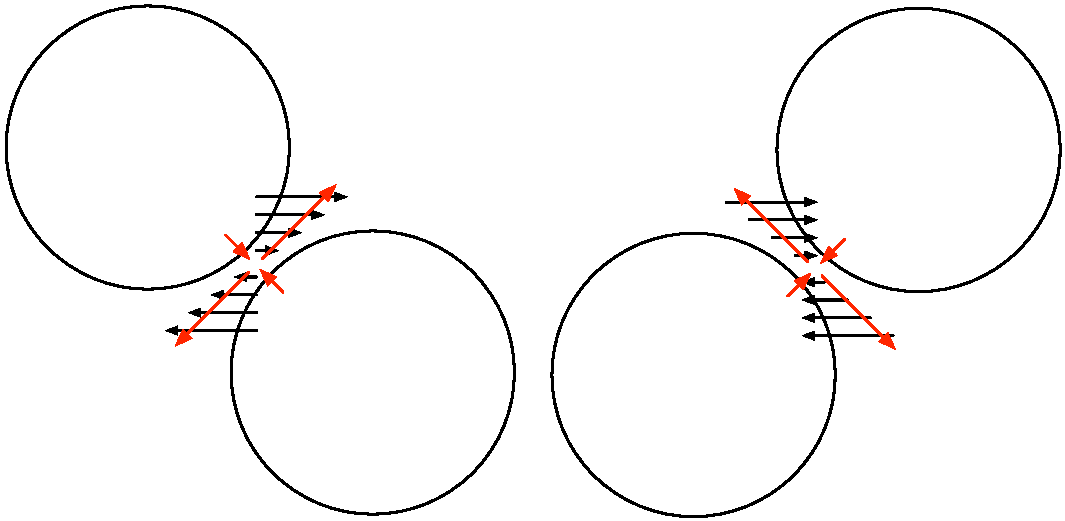
\includegraphics[width=7cm]{Lub_orientation_dependence.pdf} 
%\end{center}

\paragraph{Leading order or higher order?}

For near touching particles,
the leading terms including the $1/h$ factor
dominate to determine the particle velocities.
%
However, there seems
to be some significant differences
between the leading order lubrication force 
and full order lubrication force.

\begin{itemize}
  \item The simplified lubrication model
  includes only the squeezed mode lubrication force.
  \item 
  In the full lubrication model,
  the tangential force and torque
  diverge as $\log h^{-1}$
  \item 
  In the full lubrication model,
  the lubrication forces are depend on
  the orientation of two particles.
\end{itemize}

According to \citet{Kumar_2010a},
$\delta$-$\log\delta $ FLD gives
good agreement with SD.
%
(But, it is not clear
how good SD is in concentrated suspension.
)



\paragraph{Ball\&Melrose model}

The lubrication force used in \cite{Ball_1997}
is the leading order terms of 
the full expression given by \citet{Jeffrey_1992}.
%
In order to simulate  polydisperse system,
we need to derive 
the leading terms from \citet{Jeffrey_1992}.


\paragraph{What is singularity at $\mathrm{Pe}\to \infty$?}

\citet{Ball_1995}
and \citet{Melrose_1995}
reported singularity of pure hydrodynamic limit.
%
What is the reason for that?
%
This affects the physics?
%

\paragraph{Drag forces from background flow}

%Frame invariant pair drag model 
\citet{Ball_1997} claims that 
simulation model should satisfy frame invariant.
%
It points out that
the addition of diagonal terms corresponding to
Stokes drag forces
relative to an assumed background shear flow
breaks this frame-invariant property.
%
I don't understand why this approximation is so bad.
%
\begin{quote}
Such models are physically peculiar
because they correspond to a set of particles
each of which moves relative to the frame
of its own independently sheared fluid. 
\end{quote}

Our first model includes the diagonal terms corresponding to
Stokes drag forces.
%
As \citet{Ball_1997} pointed out,
we can expect that 
the profile of undisturbed background flow appears
in particle configuration after some shearing.
%
Stokesian dynamics has less this tendency
since the background flow can be disturbed.
\begin{figure}[htbp]
\begin{center}
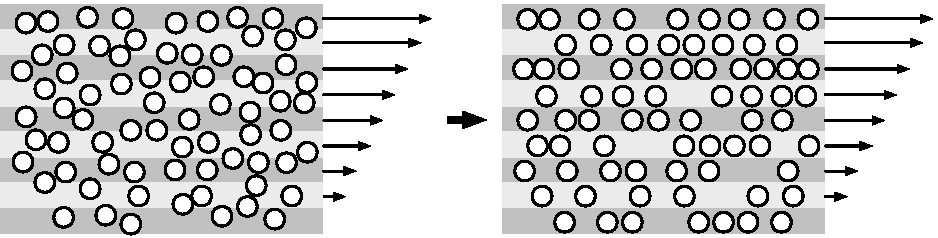
\includegraphics[width=12cm]{order_with_undisturbed_shearflow.pdf} 
\end{center}
\end{figure}

In Kumar's thesis Chapter 6 ~\citep{Kumar_2010a},
he gave some descriptions for ``fast lubrication dynamics algorithm''.
%
He investigated both, $1/\delta$ 
and $1/\delta$-$\log(1/\delta)$ lubrication models.
%
He gave three parameters for the diagonal matrix.
\begin{equation}
 \tens{R}_{\mathrm{0}}
=
\begin{pmatrix}
 R_{\mathrm{FU}}^{0} & 0 & 0 \\
 0 &  R_{\mathrm{T\Omega}}^{0}  & 0 \\
 0 &  0 &  R_{\mathrm{SE}}^{0}  
\end{pmatrix}
\end{equation}
He determined the optimal values by comparing with Stokesian dynamics.
\begin{figure}[htbp]
\centering
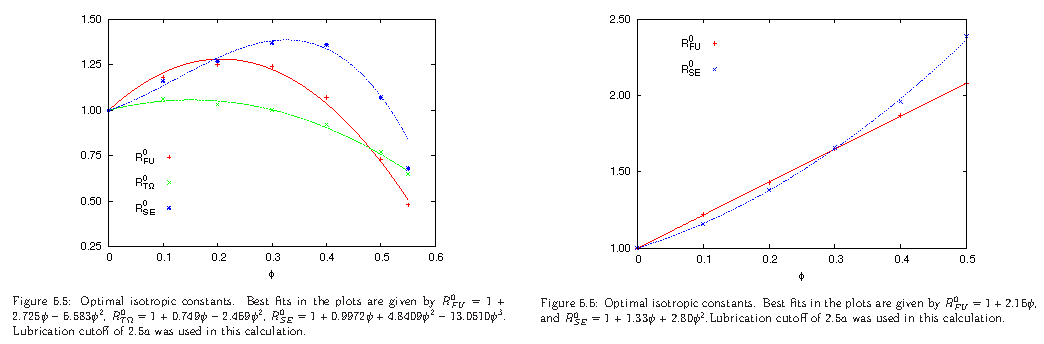
\includegraphics[width=16cm]{kumars_Rfu0.pdf} 
\caption{
Figure from Kumar's thesis.
$R_{\mathrm{FU}}^{0 }$ can be larger than 1.
%
The left one is with $\delta$-$\log \delta $ level,
and the right one with $\delta$ level,
}
\end{figure}


\begin{equation}
 \tens{R} =  \tens{R}_{\mathrm{onebody}} + \tens{R}_{\mathrm{pair}}
\end{equation}
$\tens{R}_{\mathrm{onebody}} = \tens{I}$.
\begin{align*}
\bm{F}_{\mathrm{H}} 
&=
 - \tens{R}_{\mathrm{onebody}}(\bm{U}-\bm{U}^{\infty})  
 - \tens{R}_{\mathrm{pair}}(\bm{U}-\bm{U}^{\infty})  
+  \tens{G}_{\mathrm{pair}} \tens{E}^{\infty}  
\end{align*}
%
The background flow and the drag forces acting on particles
are modeled by
$\bm{U}^{\infty}(\bm{r})$ and
the diagonal matrix $\tens{R}_{\mathrm{onebody}}$.
%

The diagonal matrix $\tens{R}_{\mathrm{onebody}}$.
%
\begin{equation}
 \tens{R}_{\mathrm{onebody}} 
= F_{\mathrm{FU}}^{0} \tens{I}
\end{equation}
%
In the dilute limit, $s$ should converge to $1$.
\begin{equation}
  s (\phi \to 0) = 1
\end{equation}

\begin{align*}
  &\bm{F}_{\mathrm{H}} = 0 \\
  & \rightarrow
  (\tens{R}_{\mathrm{onebody}} + \tens{R}_{\mathrm{pair}})(\bm{U}-\bm{U}^{\infty})  
  =  \tens{G} \tens{E}^{\infty}  
\end{align*}



\newpage

\section{Lubrication forces}

\subsection*{Jeffrey (1992)}


Interaction between particles $1$ and $2$
can be written in a linear form:
\begin{equation}
 \begin{pmatrix}
  \bm{F} \\ \bm{T} \\ \tens{S}
 \end{pmatrix}
 =
- \mu
\begin{pmatrix}
 \tens{A} &  \tilde{\tens{B}} &  \tilde{\tens{G}} \\
 \tens{B} &  \tens{C} &  \tilde{\tens{H}} \\
 \tens{G} &  \tens{H} &  \tens{M} \\
\end{pmatrix}
 \begin{pmatrix}
  \bm{U}-\bm{U}_{\infty} \\ \bm{\Omega} - \bm{\Omega}_{\infty}
 \\ -\tens{E}_{\infty}
 \end{pmatrix}
\end{equation}
Two particles are included in the expression:
\begin{equation}
 \bm{F}
= 
\begin{pmatrix}
 \bm{F}_1 \\  \bm{F}_2
\end{pmatrix}
,\quad
 \bm{T}
= 
\begin{pmatrix}
 \bm{T}_1 \\  \bm{T}_2
\end{pmatrix}
,\quad
 \tens{S}
= 
\begin{pmatrix}
 \tens{S}_1 \\  \tens{S}_2
\end{pmatrix}
,\quad
 \bm{U}
= 
\begin{pmatrix}
 \bm{U}_1 \\  \bm{U}_2
\end{pmatrix}
,\quad
 \bm{\Omega}
= 
\begin{pmatrix}
 \bm{\Omega}_1 \\  \bm{\Omega}_2
\end{pmatrix}
,\quad
 \tens{E}^{\infty}
= 
\begin{pmatrix}
  \tens{E}^{\infty} \\   \tens{E}^{\infty}
\end{pmatrix}
\end{equation}
The matrices also consist of submatrices,
e.g.~$\tens{A}$ is written as
\begin{equation}
 \tens{A}
 =
\begin{pmatrix}
  \tens{A}_{11} & \tens{A}_{12} \\
  \tens{A}_{21} & \tens{A}_{22} 
\end{pmatrix}.
\end{equation}
%
\paragraph{Variables:}
\begin{equation}
 \bm{r} \equiv \bm{r}_2 - \bm{r}_1, 
\quad
 \bm{n} \equiv \frac{\bm{r}}{r}
\end{equation}
\begin{equation}
  s \equiv \frac{2r}{a_{1}+ a_{2}}, \quad
 \lambda \equiv \frac{a_2}{a_1}, \quad
\xi \equiv s - 2
\end{equation}



\paragraph{Symmetries:}
2-indeces:
\begin{equation}
 A_{ij}^{\alpha\beta} =  A_{ji}^{\beta\alpha}
\end{equation}
3-indeces:
\begin{equation}
 G_{ijk}^{\alpha\beta} =   G_{jik}^{\alpha\beta} , \quad 
 G_{iik}^{\alpha\beta} =   H_{iik}^{\alpha\beta}  = 0, \quad 
 \tilde{G}_{ijk}^{\alpha\beta}  =  G_{jki}^{\beta\alpha} 
\end{equation}
4-indeces:
\begin{equation}
 M_{iikl}^{\alpha\beta} = 0,
\quad 
 M_{iikl}^{\alpha\beta} =  M_{lkij}^{\beta\alpha} 
\end{equation}

\paragraph{Adimensional tensors:}

The following adimensional transformation is given in \citet{Jeffrey_1984}
\begin{equation}
 \hat{\tens{A}}_{\alpha\beta}
= \frac{\tens{A}_{\alpha\beta}}{3\pi(a_{\alpha} + a_{\beta})},
\quad
 \hat{\tens{B}}_{\alpha\beta}
= \frac{\tens{B}_{\alpha\beta}}{\pi(a_{\alpha}+ a_{\beta})^2},
\quad
 \hat{\tens{C}}_{\alpha\beta}
= \frac{\tens{C}_{\alpha\beta}}{\pi(a_{\alpha}+ a_{\beta})^3}
\end{equation}

The following adimensional transformation is given in \citet{Jeffrey_1992}
\begin{equation}
 \hat{\tens{G}}_{\alpha\beta}
= \frac{\tens{G}_{\alpha\beta}}{\pi(a_{\alpha} + a_{\beta})^2},
\quad
 \hat{\tens{H}}_{\alpha\beta}
= \frac{\tens{H}_{\alpha\beta}}{\pi(a_{\alpha}+ a_{\beta})^3},
\quad
 \hat{\tens{M}}_{\alpha\beta}
= \frac{\tens{M}_{\alpha\beta}}{(5/6)\pi(a_{\alpha}+ a_{\beta})^3}
\end{equation}




\paragraph{Scalar functions}

From \citet{Jeffrey_1984}:
\begin{align}
  &\hat{A}_{ij}^{(\alpha \beta)}
   = 
  X_{\alpha \beta}^{A} n_i n_j
  +
  Y_{\alpha \beta}^{A} (\delta_{ij} - n_i n_j) \\
%%%%%%%%%%%%%%%%%%%%%%%%%%%%%%%%%%%%%%%%%%%%%%%%%%%%%%%%%%%%%%%%%%%%%%%%%%%%%%%%%%%%%%%%%%%%%%%%%%%%
  & \hat{B}_{ij}^{(\alpha \beta)}
  =
  \hat{\tilde{B}}_{ji}^{(\beta\alpha)}
  = 
  Y_{\alpha \beta}^{B}   \varepsilon_{ijk} n_k\\
%%%%%%%%%%%%%%%%%%%%%%%%%%%%%%%%%%%%%%%%%%%%%%%%%%%%%%%%%%%%%%%%%%%%%%%%%%%%%%%%%%%%%%%%%%%%%%%%%%%%
  &\hat{C}_{ij}^{\alpha \beta}
  = 
  X_{\alpha \beta}^{C} n_i n_j
  +
  Y_{\alpha \beta}^{C} (\delta_{ij} - n_i n_j)
 \approx
  X_{\alpha \beta}^{C} n_i n_j
\end{align}
From \citet{Jeffrey_1992}
\begin{align}
& \hat{G}_{ijk}^{\alpha \beta}
 = 
X_{\alpha\beta}^{G} 
\left(n_i n_j - \frac{1}{3}\delta_{ij}\right)n_k
+
Y_{\alpha\beta}^{G}
\left(
n_i \delta_{jk} + n_j \delta_{ik} - 2 n_i n_j n_k
\right) \\
%%%%%%%%%%%%%%%%%%%%%%%%%%%%%%%%%%%%%%%%%%%%%%%%%%%%%%%%%%%%%%%%%%%%%%%%%%%%%%%%%%%%%%%%%%%%%%%%%%%%
& 
\hat{H}_{ij}^{\alpha\beta}
 = Y_{\alpha\beta}^{H}
(n_i \varepsilon_{jkm} n_m 
+ n_j \varepsilon_{ikm} n_m )\\
%%%%%%%%%%%%%%%%%%%%%%%%%%%%%%%%%%%%%%%%%%%%%%%%%%%%%%%%%%%%%%%%%%%%%%%%%%%%%%%%%%%%%%%%%%%%%%%%%%%%
&
 \hat{M}_{ijkl}^{\alpha\beta}
=  \frac{3}{2}
X_{\alpha\beta}^{M}
 \left(n_i n_j
 - \frac{1}{3} \delta_{ij}
\right)
 \left(n_k n_l
 - \frac{1}{3} \delta_{kl}
\right) \\
&\qquad\qquad
+
\frac{1}{2} 
Y_{\alpha\beta}^{M}
\left(
n_i \delta_{jl} n_k
+
n_j \delta_{il} n_k
+
n_i \delta_{jk} n_l
+
n_j \delta_{ik} n_l
-
4 n_i n_j n_k n_l
\right) \\
&\qquad\qquad
+ 
\frac{1}{2}
Z_{\alpha\beta}^{M}
\left(
\delta_{ik}\delta_{jl}
+
\delta_{jk}\delta_{il}
-
\delta_{ij}\delta_{kl}
+
n_i n_j \delta_{kl} 
+
\delta_{ij} n_k n_l
+
n_i n_j n_k n_l \right.\\
&\qquad \qquad \quad
\left.
- 
n_i \delta_{jl} n_k
-
n_j \delta_{il} n_k
-
n_i \delta_{jk} n_l
-
n_j \delta_{ik} n_l
\right) 
\end{align}
\begin{align}
 X_{\alpha\beta}^{G} (s,\lambda)
& =
- X_{(3-\alpha)(3-\beta)}^{G} (s,\lambda^{-1}), \\
%%%%%%%%%%%%%%%%%%%%%%%%%%%%%%%%%%%%%%%%%%%%%%%%%%%%%%%%%%%%%%%%%%%%%%%%%%%%%%%%%%%%%%%%%%%%%%%%%%%%
 Y_{\alpha\beta}^{G} (s,\lambda)
& =
- Y_{(3-\alpha)(3-\beta)}^{G} (s,\lambda^{-1}), \\
%%%%%%%%%%%%%%%%%%%%%%%%%%%%%%%%%%%%%%%%%%%%%%%%%%%%%%%%%%%%%%%%%%%%%%%%%%%%%%%%%%%%%%%%%%%%%%%%%%%%
 Y_{\alpha\beta}^{H} (s,\lambda)
& =
 Y_{(3-\alpha)(3-\beta)}^{G} (s,\lambda^{-1}), \\
%%%%%%%%%%%%%%%%%%%%%%%%%%%%%%%%%%%%%%%%%%%%%%%%%%%%%%%%%%%%%%%%%%%%%%%%%%%%%%%%%%%%%%%%%%%%%%%%%%%%
 X_{\alpha\beta}^{M} (s,\lambda)
& =
 X_{\beta\alpha}^{M} (s,\lambda)
 =
 X_{(3-\alpha)(3-\beta)}^{M} (s,\lambda^{-1}), \\
%%%%%%%%%%%%%%%%%%%%%%%%%%%%%%%%%%%%%%%%%%%%%%%%%%%%%%%%%%%%%%%%%%%%%%%%%%%%%%%%%%%%%%%%%%%%%%%%%%%%
 Y_{\alpha\beta}^{M} (s,\lambda)
& =
 Y_{\beta\alpha}^{M} (s,\lambda)
 =
 Y_{(3-\alpha)(3-\beta)}^{M} (s,\lambda^{-1}), \\
%%%%%%%%%%%%%%%%%%%%%%%%%%%%%%%%%%%%%%%%%%%%%%%%%%%%%%%%%%%%%%%%%%%%%%%%%%%%%%%%%%%%%%%%%%%%%%%%%%%%
 Z_{\alpha\beta}^{M} (s,\lambda)
& =
 Z_{\beta\alpha}^{M} (s,\lambda)
 =
 Z_{(3-\alpha)(3-\beta)}^{M} (s,\lambda^{-1}), \\
\end{align}


The leading terms include the factor $\xi^{-1}$.
%
The leading order of scalar functions are given as follows:
%
\begin{equation*}
 g_1 (\lambda)
\approx \frac{2\lambda^2}{(1+\lambda)^3},
\quad  g_1 (1) \approx \frac{1}{4}
\end{equation*}

\begin{align}
 X_{11}^{A}
&\approx 
g_1(\lambda) \xi^{-1}, 
&  X_{11}^{A} &\approx \frac{1}{4\xi} \\
%%%%%%%%%%%%%%%%%%%%%%%%%%%%%%%%%%%%%%%%%%%%%%%%%%%%%%%%%%%%%%%%%%%%%%%%%%%%%%%%%%%%%%%%%%%%%%%%%%%%
 X_{12}^{A}
&\approx
-\frac{2}{1+\lambda}g_1(\lambda) \xi^{-1},
&
 X_{12}^{A} 
&\approx - \frac{1}{\xi} \\
%%%%%%%%%%%%%%%%%%%%%%%%%%%%%%%%%%%%%%%%%%%%%%%%%%%%%%%%%%%%%%%%%%%%%%%%%%%%%%%%%%%%%%%%%%%%%%%%%%%%
X_{11}^{C} 
& \approx 
\mathcal{O}(1) + \mathcal{O}(\xi \ln \xi^{-1}) \\
X_{12}^{C}
& \approx
\mathcal{O}(1) + \mathcal{O}(\xi \ln \xi^{-1}) \\
%%%%%%%%%%%%%%%%%%%%%%%%%%%%%%%%%%%%%%%%%%%%%%%%%%%%%%%%%%%%%%%%%%%%%%%%%%%%%%%%%%%%%%%%%%%%%%%%%%%%
 X_{11}^{G}
&\approx \frac{3}{2}g_1(\lambda) \xi^{-1}
,&
X_{11}^{G}
&\approx \frac{3}{8} \xi^{-1} \\
%%%%%%%%%%%%%%%%%%%%%%%%%%%%%%%%%%%%%%%%%%%%%%%%%%%%%%%%%%%%%%%%%%%%%%%%%%%%%%%%%%%%%%%%%%%%%%%%%%%%
 X_{12}^{G}
&\approx
\frac{-6}{(1+\lambda)^2}
g_1 (\lambda) \xi^{-1}, &
 X_{12}^{G}
&\approx
-\frac{3}{8}
 \xi^{-1},  \\
%%%%%%%%%%%%%%%%%%%%%%%%%%%%%%%%%%%%%%%%%%%%%%%%%%%%%%%%%%%%%%%%%%%%%%%%%%%%%%%%%%%%%%%%%%%%%%%%%%%%
 X_{11}^{M}
&\approx
\frac{3}{5} g_1(\lambda) \xi^{-1},
&
 X_{11}^{M}
&\approx
\frac{3}{20}  \xi^{-1}
\\
%%%%%%%%%%%%%%%%%%%%%%%%%%%%%%%%%%%%%%%%%%%%%%%%%%%%%%%%%%%%%%%%%%%%%%%%%%%%%%%%%%%%%%%%%%%%%%%%%%%%
 X_{12}^{M}
&\approx
\frac{8\lambda}{(1+\lambda)^3} g_1(\lambda) \xi^{-1}
,&
 X_{12}^{M}
&\approx
\frac{1}{4}  \xi^{-1}
\end{align}


\newpage

\paragraph{Leading order}
If we consider only the leading terms for 
the nearly contacting particles ($\xi \to 0$),
only $\tens{A}$ and $\tens{G}$ give the leading contribution to the forces.
\begin{equation}
 \begin{pmatrix}
  \bm{F}_{1} \\
  \bm{F}_{2} 
 \end{pmatrix}
\approx
- \mu
\begin{pmatrix}
\tens{A}_{11} &
\tens{A}_{12}  \\
\tens{A}_{21}  &
\tens{A}_{22}  
\end{pmatrix}
 \begin{pmatrix}
  \bm{U}_{1} -  \bm{U}_{1}^{\infty}\\
  \bm{U}_{2} -  \bm{U}_{2}^{\infty}
 \end{pmatrix}
 + \mu
\begin{pmatrix}
\tilde{\tens{G}}_{11} &
\tilde{\tens{G}}_{12}  \\
\tilde{\tens{G}}_{21}  &
\tilde{\tens{G}}_{22}  
\end{pmatrix}
 \begin{pmatrix}
\bm{E}_{\infty} \\ \bm{E}_{\infty}
\end{pmatrix}
\end{equation}

\begin{equation}
 \begin{pmatrix}
  \tens{S}_{1} \\
  \tens{S}_{2} 
 \end{pmatrix}
\approx
- \mu
\begin{pmatrix}
\tens{G}_{11} &
\tens{G}_{12}  \\
\tens{G}_{21}  &
\tens{G}_{22}  
\end{pmatrix}
 \begin{pmatrix}
  \bm{U}_{1} -  \bm{U}_{1}^{\infty}\\
  \bm{U}_{2} -  \bm{U}_{2}^{\infty}
 \end{pmatrix}
 + \mu
\begin{pmatrix}
\tens{M}_{11} &
\tens{M}_{12}  \\
\tens{M}_{21}  &
\tens{M}_{22}  
\end{pmatrix}
 \begin{pmatrix}
\bm{E}_{\infty} \\ \bm{E}_{\infty}
\end{pmatrix}
\end{equation}



\begin{align*}
F^{(1)}_i
&\approx 
- \mu A^{(11)}_{ij}
(U_{j}^{(1)}-U_{j}^{(1)\infty})
- \mu A^{(12)}_{ij}
(U_{j}^{(2)}-U_{j}^{(2)\infty})
+ \mu \tilde{G}^{(11)}_{ijk} E^{\infty}_{jk}
+ \mu \tilde{G}^{(12)}_{ijk} E^{\infty}_{jk} \\
%%%%%%%%%%%%%%%%%%%%%%%%%%%%%%%%%%%%%%%%%%%%%%%%%%%%%%%%%%%%%%%%%%%%%%%%%%%%%%%%%%%%%%%%%%%%%%%%%%%%
&=
- 6 \pi\mu a_{1} \hat{A}^{(11)}_{ij}(U_{j}^{(1)}-U_{j}^{(1)\infty})
- 3 \pi\mu (a_{1}+a_{2})\hat{A}^{(12)}_{ij} (U_{j}^{(2)}-U_{j}^{(2)\infty})\\
&\quad
+ 4 \pi\mu a_{1}^2 \hat{\tilde{G}}^{(11)}_{ijk} E^{\infty}_{jk}
+ \pi\mu (a_{1}+a_{2})^2 \hat{\tilde{G}}^{(12)}_{ijk} E^{\infty}_{jk} \\
%%%%%%%%%%%%%%%%%%%%%%%%%%%%%%%%%%%%%%%%%%%%%%%%%
&=
- 6 \pi\mu a_{1} \hat{A}^{(11)}_{ij}
(U_{j}^{(1)}-U_{j}^{(1)\infty})
- 3 \pi\mu (a_{1}+a_{2})\hat{A}^{(12)}_{ij}
(U_{j}^{(2)}-U_{j}^{(2)\infty}) \\
&\quad
+ 4 \pi\mu a_{1}^2 \hat{G}^{(11)}_{jki} E^{\infty}_{jk}
+  \pi\mu (a_{1}+a_{2})^2 \hat{G}^{(21)}_{jki} E^{\infty}_{jk} \\
%%%%%%%%%%%%%%%%%%%%%%%%%%%%%%%%%%%%%%%%%%%%%%%%%%%%%%%%%
&=
- 6 \pi\mu a_{1} X_{11}^{A}(s,\lambda) n_i n_j
(U_{j}^{(1)}-U_{j}^{(1)\infty})
- 3 \pi\mu (a_{1}+a_{2}) X_{12}^{A}(s,\lambda) n_i n_j
(U_{j}^{(2)}-U_{j}^{(2)\infty}) \\
&\quad
+ 4 \pi\mu a_{1}^2 X_{11}^{G}(s,\lambda) 
n_i\left(n_j n_k - \frac{\delta_{jk}}{3}  \right) E^{\infty}_{jk}
+  \pi\mu (a_{1}+a_{2})^2
X_{21}^{G}(s,\lambda) 
n_i\left(n_j n_k - 
\frac{\delta_{jk}}{3} \right) E^{\infty}_{jk} \\
%%%%%%%%%%%%%%%%%%%%%%%%%%%%%%%%%%%%%%%%%%%%%%%%%%%%%%%%%%%%%%%%%%%%%%%%%%%%%%%%%%%%%%%%%%%%%%%%%%%%
&=
- 6 \pi\mu a_{1} X_{11}^{A}(s,\lambda) n_i n_j
(U_{j}^{(1)}-U_{j}^{(1)\infty})
- 3 \pi\mu (a_{1}+a_{2}) X_{12}^{A}(s,\lambda) n_i n_j
(U_{j}^{(2)}-U_{j}^{(2)\infty}) \\
&\quad
+ 4 \pi\mu a_{1}^2 X_{11}^{G} (s,\lambda)
n_i\left(n_j n_k - \frac{\delta_{jk}}{3}  \right) E^{\infty}_{jk}
-  \pi\mu (a_{1}+a_{2})^2 X_{12}^{G}(s,\lambda^{-1})
n_i\left(n_j n_k - 
\frac{\delta_{jk}}{3} \right) E^{\infty}_{jk} \\
%%%%%%%%%%%%%%%%%%%%%%%%%%%%%%%%%%%%%%%%%%%
&=
6 \pi\mu
\left(
-  a_{1} \frac{g_1(\lambda)}{\xi} n_i n_j
(U_{j}^{(1)}-U_{j}^{(1)\infty})
+ \frac{a_{1}+a_{2}}{1+\lambda} \frac{g_1(\lambda)}{\xi} n_i n_j
(U_{j}^{(2)}-U_{j}^{(2)\infty})\right.
\\
&\quad + 
\left.
 a_{1}^2 \frac{g_1(\lambda)}{\xi} 
n_i\left(n_j n_k - \frac{\delta_{jk}}{3} \right) E^{\infty}_{jk}
+  
\frac{  \lambda^2}{(1+\lambda)^2} 
 (a_{1}+ a_{2})^2
\frac{g_1(1/\lambda)}{\xi} n_i\left(n_j n_k 
- \frac{\delta_{jk}}{3} \right)E^{\infty}_{jk} 
\right)
\end{align*}

\begin{itemize}
 \item $\tilde{G}_{ijk}^{(11)}=G_{jki}^{(11)}$,
$\tilde{G}_{ijk}^{(12)}=G_{jki}^{(21)}$,
$\tilde{G}_{ijk}^{(21)}=G_{jki}^{(12)}$,
$\tilde{G}_{ijk}^{(22)}=G_{jki}^{(22)}$.

 \item 
$X_{11}^{G}(s,\lambda)
= - X_{22}^{G} (s, \lambda^{-1})$
and $X_{21}^{G}(s,\lambda)
= - X_{12}^{G} (s, \lambda^{-1})$

 \item 
$X_{11}^{A}(s,\lambda)\approx g_1(\lambda) \frac{1}{\xi}$, 
$X_{12}^{A}(s,\lambda) \approx -\frac{2}{1+\lambda}g_1(\lambda) \frac{1}{\xi}$\\
$X_{11}^{G}(s,\lambda)\approx \frac{3}{2} g_1(\lambda) \frac{1}{\xi}$,
$X_{12}^{G}(s,\lambda)\approx -\frac{6}{(1+\lambda)^2} g_1(\lambda) \frac{1}{\xi}$   
\end{itemize}
Monodisperse $a_\alpha = a_{\beta}=a$, $g_1(1)=1/4$.
\begin{align}
 F^{(1)}_i
&= 
\frac{6 \pi\mu a}{4\xi}
\left(
-   n_i n_j
(U_{j}^{(1)}-U_{j}^{(1)\infty})
+   n_i n_j
(U_{j}^{(2)}-U_{j}^{(2)\infty})
+  
2a n_i\left\{n_j n_k - \frac{\delta_{jk}}{3} \right\} E^{\infty}_{jk}
\right) \notag \\
&= 
-
\frac{3 \pi\mu a}{2\xi}
\left(
   n_i n_j
(U_{j}^{(1)}-U_{j}^{(1)\infty})
-   n_i n_j
(U_{j}^{(2)}-U_{j}^{(2)\infty})
-  
2a n_in_j  E^{\infty}_{jk}n_k
+2an_i(E^{\infty}_{xx}+E^{\infty}_{yy}+E^{\infty}_{zz} )
\right)
\end{align}

cf. Ball\&Melrose expression:
\begin{equation}
F_i^{(1)}
=
- 
\frac{3 \pi \mu a^2}{2 h_{\ij}}
\left(
n_{i} n_j (U^{(1)}_j-U^{(1)\infty}_j)
- n_{i} n_j (U^{(2)}_j-U^{(2)\infty}_j)
- (2+h/a) n_i n_j  E_{jk}n_k
\right) 
 \end{equation}

\subsection{Approximation for leading-order of lubrication}


\begin{equation}
 \begin{pmatrix}
  \bm{F}_{1} \\
  \bm{F}_{2} 
 \end{pmatrix}
\approx
- \mu
\begin{pmatrix}
\tens{A}_{11} &
\tens{A}_{12}  \\
\tens{A}_{21}  &
\tens{A}_{22}  
\end{pmatrix}
 \begin{pmatrix}
  \bm{U}_{1} -  \bm{U}_{1}^{\infty}\\
  \bm{U}_{2} -  \bm{U}_{2}^{\infty}
 \end{pmatrix}
 + \mu
\begin{pmatrix}
\tilde{\tens{G}}_{11} &
\tilde{\tens{G}}_{12}  \\
\tilde{\tens{G}}_{21}  &
\tilde{\tens{G}}_{22}  
\end{pmatrix}
 \begin{pmatrix}
\bm{E}_{\infty} \\ \bm{E}_{\infty}
\end{pmatrix}
\end{equation}

\begin{equation}
 \begin{pmatrix}
  \tens{S}_{1} \\
  \tens{S}_{2} 
 \end{pmatrix}
\approx
- \mu
\begin{pmatrix}
\tens{G}_{11} &
\tens{G}_{12}  \\
\tens{G}_{21}  &
\tens{G}_{22}  
\end{pmatrix}
 \begin{pmatrix}
  \bm{U}_{1} -  \bm{U}_{1}^{\infty}\\
  \bm{U}_{2} -  \bm{U}_{2}^{\infty}
 \end{pmatrix}
 + \mu
\begin{pmatrix}
\tens{M}_{11} &
\tens{M}_{12}  \\
\tens{M}_{21}  &
\tens{M}_{22}  
\end{pmatrix}
 \begin{pmatrix}
\bm{E}_{\infty} \\ \bm{E}_{\infty}
\end{pmatrix}
\end{equation}


\paragraph{XA}
\begin{equation}
 g_1 (\lambda) = \frac{2\lambda^2}{(1+\lambda)^3}
\end{equation}

$X_{\alpha\beta}^{A}(s,\lambda)=X_{\beta\alpha}^{A}(s,\lambda) =
X_{(3-\alpha)(3-\beta)}^{A}(s,\lambda^{-1})$
\begin{align}
 X_{11}^{A}(s,\lambda) &= g_1 (\lambda) \xi^{-1} \\
 X_{12}^{A}(s,\lambda) &= - \frac{2}{1+\lambda} g_1 (\lambda) \xi^{-1} 
= -\frac{2}{1+\lambda} X_{11}^{A}(s,\lambda) \\
 X_{21}^{A}(s,\lambda) &=  X_{12}^{A}(s,\lambda) \\
 X_{22}^{A}(s,\lambda) &=  X_{11}^{A}(s,\lambda^{-1}) 
 = g_1(\lambda^{-1})\xi^{-1}
 = \frac{1}{\lambda} g_1(\lambda) \xi^{-1}
 = \frac{1}{\lambda} X_{11}^{A}(s,\lambda) 
\end{align}

\paragraph{XG}
$X_{\alpha\beta}^{G}(s,\lambda) = - X_{(3-\alpha)(3-\beta)}^{G}(s, \lambda^{-1})$
\begin{align}
 X_{11}^{G}(s,\lambda) &= \frac{3}{2}g_1(\lambda) \xi^{-1} \\
 X_{22}^{G}(s,\lambda) &= - X_{11}^{G} (s, \lambda^{-1})
 = - \frac{3}{2}g_1(\lambda^{-1}) \xi^{-1} 
 = - \frac{1}{\lambda} \frac{3}{2}g_1(\lambda) \xi^{-1} 
 = - \frac{1}{\lambda} X_{11}^{G} (s, \lambda) \\
X_{12}^{G}(s,\lambda) &= 
-\frac{6}{(1+\lambda)^2} g_1(\lambda)\xi^{-1} 
= 
-\frac{6}{(1+\lambda)^2} \frac{2}{3} X_{11}^{G}(s,\lambda)
= 
-\frac{4}{(1+\lambda)^2}  X_{11}^{G} (s,\lambda)\\
X_{21}^{G}(s,\lambda) &= 
- X_{12}^{G}(s,\lambda^{-1}) 
= 
\frac{4}{(1+\lambda^{-1})^2}X_{11}^{G}(s,\lambda^{-1})
= 
-\frac{4}{(1+\lambda^{-1})^2}X_{22}^{G}(s,\lambda)
\end{align}

\paragraph{XM}

$X_{\alpha\beta}^{M} (s,\lambda) = 
 X_{\beta\alpha}^{M}(s,\lambda) = 
 X_{(3-\alpha)(3-\beta)}^{M}(s, \lambda^{-1})$

\begin{align}
X_{11}^{M}(s,\lambda)  &= 
\frac{3}{5} g_1(\lambda)\xi^{-1} \\
X_{12}^{M}(s,\lambda)
&= \frac{8\lambda}{(1+\lambda)^3} g_1(\lambda)\xi^{-1} 
= \frac{40\lambda}{3(1+\lambda)^3}  X_{11}^{M}(s,\lambda) \\
X_{21}^{M}(s,\lambda) & = X_{12}^{M}(s,\lambda) \\
X_{22}^{M}(s,\lambda) & = 
X_{11}^{M}(s,\lambda^{-1}) 
=
\frac{3}{5} g_1(\lambda^{-1})\xi^{-1} 
=
\frac{1}{\lambda}
\frac{3}{5} g_1(\lambda)\xi^{-1} 
=
\frac{1}{\lambda}
X_{11}^{M}(s,\lambda)  
\end{align}


\begin{align}
\frac{1}{6\pi} F^{\alpha}_i
&= -n_i \left(
a_{\alpha} X_{\alpha\alpha}^{A} \Delta v^{\alpha}_j
+ \frac{r_0}{2} 
X_{\alpha\beta}^{A} n_j \Delta v^{\beta}_j
\right) 
 +
\dot{\gamma}
\left( \frac{2}{3} a_{\alpha}^2   X_{\alpha\alpha}^{G} 
 + \frac{r_0^2}{6} X_{\alpha\beta}^{G} \right)n_z n_x  n_i \\
\frac{1}{6\pi} F^{\alpha}_i
&= -n_i \left(
a_{\alpha} X_{\alpha\alpha}^{A} \Delta v^{\alpha}_j
+ \frac{r_0}{2} 
X_{\alpha\beta}^{A} n_j \Delta v^{\beta}_j
\right)
 + 
\dot{\gamma}
\left( \frac{2}{3} a_{\beta}^2 X_{\alpha\alpha}^{G}
  + \frac{r_0^2}{6} X_{\alpha\beta}^{G}\right)
n_z n_x n_i
\end{align}

\begin{align}
\tens{S}_1
 = 
- \mu \tens{G}_{11} (\bm{U}_1-\bm{U}_1^{\infty})
- \mu \tens{G}_{12} (\bm{U}_2-\bm{U}_2^{\infty})
+ \mu \tens{M}_{11} \tens{E}_{\infty}
+ \mu \tens{M}_{12} \tens{E}_{\infty}
\end{align}

\begin{gather}
 \hat{G}_{ijk}^{\alpha \beta}
\approx 
X_{\alpha\beta}^{G} 
\left(n_i n_j - \frac{1}{3}\delta_{ij}\right)n_k\\
 \hat{\tens{G}}_{\alpha\beta}
= \frac{\tens{G}_{\alpha\beta}}{\pi(a_{\alpha} + a_{\beta})^2},
\end{gather}
\begin{align}
 G^{11}_{ijk} (\Delta U^{1}_k)
+ G^{12}_{ijk} (\Delta U^{2}_k)
&= c_{11} \hat{G}^{11}_{ijk} (\Delta U^{1}_k)
+ c_{12} \hat{G}^{12}_{ijk} (\Delta U^{2}_k) \\
&= c_{11} X_{11}^{G}(n_i n_j - \frac{1}{3}\delta_{ij}) n_k (\Delta U^{1}_k)
+ c_{12} X_{12}^{G}(n_i n_j - \frac{1}{3}\delta_{ij}) n_k  (\Delta U^{2}_k) \\
&=
(n_i n_j - \frac{1}{3}\delta_{ij}) n_k
\left(
\pi 4 a_1^2 X_{11}^{G} (\Delta U^{1}_k)
+ 
\pi (a_1+a_2)^2 X_{12}^{G} (\Delta U^{2}_k)
\right)
\end{align}

\begin{align}
\frac{1}{6\mu\pi} 
\left\{
 S^{1}_{ij}
\right\}_{U}
= - 
(n_i n_j - \frac{1}{3}\delta_{ij}) n_k
\left(
 \frac{2}{3} a_1^2 X_{11}^{G} (\Delta U^{1}_k)
+ 
\frac{1}{6}
 (a_1+a_2)^2 X_{12}^{G} (\Delta U^{2}_k)
\right)
\end{align}



\begin{equation}
 \hat{M}_{ijkl}^{\alpha\beta}
=  \frac{3}{2}
X_{\alpha\beta}^{M}
 \left(n_i n_j
 - \frac{1}{3} \delta_{ij}
\right)
 \left(n_k n_l
 - \frac{1}{3} \delta_{kl}
\right)  
\end{equation}


\begin{align*}
\left\{
S^{\alpha}_{ij}
\right\}_{E\alpha\beta}
&= 
c \hat{M}_{ijkl}^{\alpha\beta} E_{kl}^{\infty} \\
&=
c (
\hat{M}_{ijkx}^{\alpha\beta} E_{kx}^{\infty}
+
\hat{M}_{ijky}^{\alpha\beta} E_{ky}^{\infty}
+
\hat{M}_{ijkz}^{\alpha\beta} E_{kz}^{\infty}) \\
&=
c (
\hat{M}_{ijxx}^{\alpha\beta} E_{xx}^{\infty}
+
\hat{M}_{ijyx}^{\alpha\beta} E_{yx}^{\infty}
+
\hat{M}_{ijzx}^{\alpha\beta} E_{zx}^{\infty} \\
&\quad 
+
\hat{M}_{ijxy}^{\alpha\beta} E_{xy}^{\infty}
+
\hat{M}_{ijyy}^{\alpha\beta} E_{yy}^{\infty}
+
\hat{M}_{ijzy}^{\alpha\beta} E_{zy}^{\infty} \\
&\quad 
+
\hat{M}_{ijxz}^{\alpha\beta} E_{xz}^{\infty}
+
\hat{M}_{ijyz}^{\alpha\beta} E_{yz}^{\infty} 
+
\hat{M}_{ijzz}^{\alpha\beta} E_{zz}^{\infty}) \\
&=
c(
\hat{M}_{ijzx}^{\alpha\beta}
+
\hat{M}_{ijxz}^{\alpha\beta}
) E_{zx}^{\infty} 
=
2c\hat{M}_{ijxz}^{\alpha\beta}  E_{xz}^{\infty} \\
&=
3c X_{\alpha\beta}^{M}
(n_i n_j-\frac{1}{3}\delta_{ij}) 
n_x n_z E_{xz}^{\infty} 
\end{align*}


\begin{align}
\left\{
S_{ij}^{1}
\right\}_{\mathrm{E}}
 &= 
 3 c_{11} X_{11}^{M}
(n_i n_j-\frac{1}{3}\delta_{ij}) 
n_x n_z E_{xz}^{\infty} 
+
3 c_{12 }X_{12}^{M}
(n_i n_j-\frac{1}{3}\delta_{ij}) 
n_x n_z E_{xz}^{\infty}  \\
&= 3 (
c_{11} X_{11}^{M}
+ 
c_{12} X_{12}^{M})
(n_i n_j-\frac{1}{3}\delta_{ij})
n_x n_z E_{xz}^{\infty} 
 \\
&= 3 (
\frac{5\pi}{3} 4 a_1^3 X_{11}^{M}
+ 
\frac{5\pi}{6} (a_1 + a_2)^3 X_{12}^{M})
(n_i n_j-\frac{1}{3}\delta_{ij})
n_x n_z E_{xz}^{\infty} 
 \\
&=  (
20\pi  a_1^3  X_{11}^{M}
+ 
\frac{5}{2}\pi (a_1+a_2)^3 X_{12}^{M})
(n_i n_j-\frac{1}{3}\delta_{ij}) 
n_x n_z \frac{\dot{\gamma}}{2}
\end{align}

\begin{align*}
\left\{
\frac{1}{6\mu\pi} S_{ij}^{1} 
\right\}_{E}
&= 
  (
\frac{10}{3}  a_1^3  X_{11}^{M}
+ 
\frac{5}{12} (a_1+a_2)^3 X_{12}^{M})
(n_i n_j-\frac{1}{3}\delta_{ij}) 
n_x n_z \frac{\dot{\gamma}}{2}
\\
&=
  (
\frac{5}{3}  a_1^3  X_{11}^{M}
+ 
\frac{5}{24} (a_1+a_2)^3 X_{12}^{M})
(n_i n_j-\frac{1}{3}\delta_{ij}) 
n_x n_z \dot{\gamma}
\end{align*}

$\tens{M}_{11} \bm{E}_{\infty}$

\begin{equation}
  X_{11}^{M}
\approx
\frac{3}{5} g_1(\lambda) \xi^{-1},
%%%%%%%%%%%%%%%%%%%%%%%%%%%%%%%%%%%%%%%%%%%%%%%%%%%%%%%%%%%%%%%%%%%%%%%%%%%%%%%%%%%%%%%%%%%%%%%%%%%%
 X_{12}^{M}
\approx
\frac{8\lambda}{(1+\lambda)^3} g_1(\lambda) \xi^{-1}
\end{equation}


%\begin{align}
%\frac{ F^{\alpha}_i}{F_0}
%&= 
%-  \frac{1}{4\xi} n_i n_j
%(\bm{U}_{\alpha}-\bm{U}_{\alpha}^{\infty})_j
%+ \frac{1}{4\xi} n_i n_j
%(\bm{U}_{\beta}-\bm{U}_{\beta}^{\infty})_j 
%\\
%&\quad
%+ \frac{3}{8\xi}
%(n_i n_j - 1/3 \delta_{ij}) \bm{E}^{\infty}_{jk}
%-  
%\frac{3}{8\xi}
%(n_i n_j - 1/3 \delta_{ij}) \bm{E}^{\infty}_{jk} 
%\end{align}


\newpage

\section{Singularity?}

\begin{equation}
 \bm{F}^{(i,j)} = \frac{1}{4h}(\bm{v}^{(i)} - \bm{v}^{(j)})\cdot \bm{n} \bm{n}
\end{equation}
and the force balance equation,
\begin{equation}
 \bm{F}^{(i)} = 
\sum_j
 \bm{F}^{(i,j)} = 0
\end{equation}
we can find the solutions $\bm{v}^{(i)}$ ($i=1,\dotsc,n$).
%
However,
the gaps between particles 
become smaller and smaller 
due to many-body interactions (pileup compression).
%
In this case,
accurate orbits requires infinite precision.
%
But, numerical simulation can deal with finite precision,
and the time integration is approximation (i.e. Euler method or something similar).
%
This always generate inaccurate evaluation of the stresslet.







\section{Ball\&Melrose model}

One-body limit:
\begin{align}
 \bm{F}_i^{\mathrm{self}} &= 
-6 \pi \mu a ( \bm{v}_i - \bm{U}^{\infty} (\bm{r}_i) ) \\
 \bm{T}_i^{\mathrm{self}} &= 
-8 \pi \mu a^3 ( \bm{\omega}_i - \bm{\Omega}^{\infty})
\end{align}
%
\citet{Melrose_2004a} used
the leading squeeze mode of lubrication force:
\begin{align}
 \bm{F}_{ij}^{\mathrm{pair}}
&=
- \alpha_{\mathrm{n}}(h_{ij})
\bigl\{
(\bm{v}_i - \bm{v}_j)
\cdot \bm{n}_{ij}
\bigr\}
\bm{n}_{ij} \\
 \bm{T}_{ij}^{\mathrm{pair}}
&=
\bm{0},
\end{align}
where
\begin{equation}
 \alpha_{\mathrm{n}}(h_{ij}) = 
\frac{3 \pi \mu a^2}{2 h_{\ij}}.
\end{equation}
Hydrodynamic interaction acting on particle $i$
is given by
\begin{align}
\bm{F}_i^{\mathrm{H}}
&=
\bm{F}_i^{\mathrm{self}}
+
\sum_j
\bm{F}_{ij}^{\mathrm{pair}} \\
\bm{T}_i^{\mathrm{H}}
&=
\bm{T}_i^{\mathrm{self}}
\end{align}


\subsection*{Dimensionless equations}

The unit of length, velocity and force 
are given:
$L_0 = a$,  $v_0 = a \dot{\gamma}$, and $F_0 \equiv 6 \pi \mu a v_0$.

The dimensionless variables are introduced:
$\tilde{h}_{ij} = h_{ij} / L_0$,
$\tilde{\bm{v}}_i = \bm{v}_i / U_0$,
and $\tilde{\bm{F}}_{ij}^{\mathrm{pair}} = \bm{F}_{ij}^{\mathrm{pair}} / F_0$.

The relations are written as follows:
\begin{equation}
 \tilde{\bm{F}}_i^{\mathrm{self}} = 
-( \tilde{\bm{v}}_i - 
\tilde{\bm{U}}^{\infty} 
(\tilde{\bm{r}}_i) )
\end{equation}
\begin{equation}
 \tilde{\bm{F}}_{ij}^{\mathrm{pair}}
= 
- \frac{1}{4 \tilde{h}_{ij}}
\bigl\{
(\tilde{\bm{v}}_i-
\tilde{\bm{v}}_i)\cdot
\bm{n}_{ij}
\bigr\}\bm{n}_{ij}
\end{equation}

\begin{equation}
 \bm{U}^{\infty}(\bm{r})
 = 
 \dot{\gamma} z \bm{e}_{x}
\end{equation}
\begin{equation}
\Longrightarrow
  \tilde{\bm{U}}^{\infty}(\tilde{\bm{r}})
 = 
 \dot{\gamma} z \bm{e}_{x} / U_0
=  \dot{\gamma} z \bm{e}_{x} / (\dot{\gamma} a)
= \tilde{z} \bm{e}_{x} 
\end{equation}


\subsection*{Matrix form}
\begin{align*}
 \bm{F}_{\alpha\beta}^{\mathrm{pair}}
&= 
- \frac{1}{4 h_{\alpha\beta}}
\bigl\{
(\bm{v}_\alpha-
\bm{v}_\beta)\cdot
\bm{n}_{\alpha\beta}
\bigr\}\bm{n}_{\alpha\beta} \\
&=
- \frac{1}{4 h_{\alpha\beta}}
\Bigl[
\bigl\{
(\bm{v}_\alpha- \bm{U}^{\infty}_\alpha)-
(\bm{v}_\beta- \bm{U}^{\infty}_\beta)
+ \bm{U}^{\infty}_\alpha
- \bm{U}^{\infty}_\beta
\bigr\}\cdot
\bm{n}_{\alpha\beta}
\Bigr]
\bm{n}_{\alpha\beta}
\end{align*}


$\Delta \bm{v} \equiv (\bm{v}- \bm{U}^{\infty})$
\begin{align*}
\Delta \bm{v} \cdot
\bm{n} \bm{n}
= &
(\Delta v_x n_x 
+\Delta v_y n_y
+\Delta v_z n_z) n_x \bm{i}\\
& 
+ (\Delta v_x n_x 
+\Delta v_y n_y
+\Delta v_z n_z) n_y \bm{j}\\
&
+ (\Delta v_x n_x 
+\Delta v_y n_y
+\Delta v_z n_z) n_z \bm{k} \\
=&
\begin{pmatrix}
 n_x n_x &   n_y n_x &   n_z n_x \\
 n_x n_y &   n_y n_y &   n_z n_y \\
 n_x n_z &   n_y n_z &   n_z n_z 
\end{pmatrix}
\begin{pmatrix}
 \Delta v_x \\
 \Delta v_y \\
 \Delta v_z 
\end{pmatrix} 
\end{align*}
\begin{equation*}
(\Delta \bm{v} \cdot
\bm{n} \bm{n})_i
= n_i n_j \Delta v_j
\end{equation*}


\begin{align*}
  \bm{F}_\alpha  &= 
  -  \Delta \bm{v}_\alpha
  - \sum_{\beta}
  \frac{1}{4h_{\alpha\beta}}
  \left(
    \bm{n}_{\alpha\beta} (\bm{n}_{\alpha\beta}\cdot \Delta \bm{v}_{\alpha})
    - 
    \bm{n}_{\alpha\beta} (\bm{n}_{\alpha\beta}\cdot \Delta \bm{v}_\beta )
    +
    \bm{n}_{\alpha\beta}
    \left\{
      \bm{n}_{\alpha\beta}  \cdot
      (\bm{U}_{\alpha}^{\infty}-\bm{U}_{\beta}^{\infty})
    \right\}
  \right)  \\
&=  -  \Delta \bm{v}_\alpha 
 - \sum_{\beta}
  \frac{1}{4h_{\alpha\beta}}
  \left(
    \bm{n}_{\alpha\beta} (\bm{n}_{\alpha\beta}\cdot \Delta \bm{v}_{\alpha})
    - 
    \bm{n}_{\alpha\beta} (\bm{n}_{\alpha\beta}\cdot \Delta \bm{v}_\beta )
    +
    \bm{n}_{\alpha\beta}
    \left\{
  ....
    \right\}
  \right) \\
&=  -  \Delta \bm{v}_\alpha 
 - \sum_{\beta}
  \frac{1}{4h_{\alpha\beta}}
  \left(
    \bm{n}_{\alpha\beta} (\bm{n}_{\alpha\beta}\cdot \Delta \bm{v}_{\alpha})
    - 
    \bm{n}_{\alpha\beta} (\bm{n}_{\alpha\beta}\cdot \Delta \bm{v}_\beta )
    -
r_{\alpha\beta}
  \bm{n}_{\alpha\beta}
  \left\{
\bm{n}_{\alpha\beta} \cdot
(\tens{E}^{\infty} \bm{n}_{\alpha\beta})
    \right\} 
  \right) 
\end{align*}
$\bm{n}_{\alpha\beta} = \bm{r}^{\beta}-\bm{r}^{\alpha}$
\begin{align*}
    \bm{n}_{\alpha\beta}    \left\{
  ....
    \right\} &= 
  \bm{n}_{\alpha\beta}
  \left\{
    \bm{n}_{\alpha\beta}  \cdot
      (
\Omega^{\infty} \times (\bm{r}^{\alpha}-\bm{r}^{\beta})
+ 
\tens{E}^{\infty}
(\bm{r}^{\alpha}-\bm{r}^{\beta}))
)
    \right\} \\
&= 
r_{\alpha\beta}
  \bm{n}_{\alpha\beta}
  \left\{
      (
\bm{n}_{\alpha\beta} \cdot \Omega^{\infty} \times \bm{n}_{\alpha\beta}
- 
\bm{n}_{\alpha\beta} \cdot
(\tens{E}^{\infty} \bm{n}_{\alpha\beta})
)
    \right\} \\
&= 
-r_{\alpha\beta}
  \bm{n}_{\alpha\beta}
  \left\{
\bm{n}_{\alpha\beta} \cdot
(\tens{E}^{\infty} \bm{n}_{\alpha\beta})
    \right\} 
\end{align*}

\begin{align*}
 F^{\alpha}_i
&=
- \Delta v^{\alpha}_i
- \frac{1}{4 h}
\left(
n_{i} n_j \Delta v^{\alpha}_j
- n_{i} n_j \Delta v^{\beta}_j
- r n_i n_j n_k E_{jk}
\right) \\
&=
- \Delta v^{\alpha}_i
- \frac{1}{4 h}
\left(
n_{i} n_j \Delta v^{\alpha}_j
- n_{i} n_j \Delta v^{\beta}_j
- r n_i n_j n_k E_{jk}
\right) 
\end{align*}






\begin{align}
\begin{pmatrix}
\vdots \\ \bm{F}_i \\ \vdots \\ \bm{F}_j \\  \vdots  
\end{pmatrix}
& =
\begin{pmatrix}
\vdots \\
\bm{F}_{i}^{\mathrm{self}} +  \bm{F}_{ij}^{\mathrm{pair}}  
\\ \vdots \\ 
\bm{F}_{j}^{\mathrm{self}} +  \bm{F}_{ji}^{\mathrm{pair}}  
\\  \vdots  
\end{pmatrix} \\
&=
-
\begin{pmatrix}
\cdots & \cdots & \cdots & \cdots & \cdots\\
\cdots & 1 + \frac{1}{4h_{ij}}\bm{n}_{ij} \otimes \bm{n}_{ij}  
& \cdots & -\frac{1}{4h_{ij}}\bm{n}_{ij} \otimes \bm{n}_{ij}   & \cdots\\
\cdots & \cdots & \cdots & \cdots & \cdots\\
\cdots & -\frac{1}{4h_{ji}}\bm{n}_{ji} \otimes \bm{n}_{ji} & \cdots 
& 1 + \frac{1}{4h_{ji}}\bm{n}_{ji} \otimes \bm{n}_{ji} 
 & \cdots \\
\cdots & \cdots & \cdots & \cdots & \cdots 
\end{pmatrix}
\begin{pmatrix}
\vdots \\
\Delta \bm{v}_i \\ 
\vdots \\
\Delta \bm{v}_j \\
\vdots 
\end{pmatrix} \\
& \quad 
+ 
\begin{pmatrix}
\vdots \\
-\frac{1}{4h_{ij}}
 \frac{(z_i - z_j )(x_i-x_j)}{r_{ij}} 
 \bm{n}_{ij} \\
\vdots \\
-\frac{1}{4h_{ji}} 
 \frac{(z_j - z_i )(x_j - x_i)}{r_{ji}} 
\bm{n}_{ji} \\
\vdots 
\end{pmatrix} 
\end{align}




\bibliography{/Users/seto/Dropbox/Papers/rse}
\end{document}